\documentclass[11pt, a4paper, twocolumn]{article}

\usepackage[utf8]{inputenc}
\usepackage[]{biblatex} % References
\usepackage[hidelinks]{hyperref} % Clickable links
\usepackage{url} % Wrap urls
\usepackage{siunitx} % Typeset units
\usepackage{graphicx} % Import graphics

\graphicspath{{graphics/}}

\sisetup{per-mode=symbol} % (siunitx) Use symbols for 'per' values e.g. m/s
\DeclareSIUnit\feet{ft} % Add the imperial 'feet' unit
\newcommand{\hPa}{\hecto\pascal} % Shorter command for hPa

\bibliography{refs.bib}

\title{Using Smart Devices as Tools in Safety Critical Skydiving Applications}
\author{Christopher Lane}

\begin{document}
\maketitle

\begin{abstract} % "Helps decide if someone should read the paper"
    Smart devices such as smartphones and smartwatches today have many different sensors, often with high frequency and accuracy. One sensor that is becoming more common in smart devices is the barometer, this allows for air pressure to be measured, making altitude calculations possible. Since skydiving equipment is typically expensive, it would be useful for skydivers to enhance their skydiving experience using the smart devices that they already own. This article will discuss how an app might be created to give guidance to a skydiver to improve their canopy piloting.
\end{abstract}

\section{Introduction}\label{sec:introduction} % "Lays out the whole paper"

% What is the problem?
Learning to skydive is a fast learning curve, and in particular, the journey under canopy (parachute) is arguably the most dangerous part of the skydive. A skydiver must ensure they avoid all obstacles such as other skydivers, guide themselves to a safe landing area and avoid making any dangerous low turns. Student skydivers often struggle to predict their trajectory while planning their landing pattern and this can result in landing far from the intended landing area or taking dangerous actions in an attempt to meet their target area.
Skydiving gear is costly; this makes sense because there are not a tremendous amount of manufacturers and everything that is created is safety-critical and specialised. There are no tools beyond radio communication with an instructor on the ground to aid student's with their canopy skills, and even this is usually not used after the first two jumps.

% Why is the problem important?
The problem to be solved is important because there are substantial safety concerns when skydiving students are flying their canopies and little to aid them to fly better and safer other than with pre and post skydive training.

% What has been done so far on the problem?
So far there has been very little done to solve the problem of helping student skydivers improve their landing patterns and be safer in the sky during the activity; all of the support takes place on the ground.

% What is the contribution of this paper to the problem?
This paper proposes a proof-of-concept app to aid skydivers before, during and after a skydive, focussing primarily on features to improve landing pattern accuracy and safety.
An investigation has been documented in the appropriateness of today's smart devices such as smartphones and smartwatches for use in safety-critical skydiving applications.

% Is the contribution original? Explain why
Through our research, we have found that this problem does not appear to have been tackled before. Very few apps exist already for gliding air sports such as paragliding but these only provide simple statistics such as current altitude and speed, nothing could be found to provide live feedback or safety-enhancing features.

% Is the contribution non-trivial? Explain why
This project will contribute solutions to the problems skydivers face. The project will solve significant challenges such as how to calculate and recommend a landing pattern that can be used to guide a skydiver to their landing area with a higher degree of accuracy, all while ensuring skydiving safety measures are maintained. The challenge of calculating landing patterns becomes especially tricky when it must also adjust to live, changing data. Other challenges that will be explained in the paper include being able to detect other skydivers in the sky to produce collision warnings and being able to present collected jump data to a skydiver in a way that is intuitive and can be used for learning.

% Short summary of the rest of the paper
The rest of the paper is structured as follows: In Section~\ref{sec:related-work} we explore existing work that can be used to gain an understanding on the current state of research into solutions to problems that we will face. In Section~\ref{sec:theory}, the theory will be explained that will be required knowledge when creating a solution to the problem. Section~\ref{sec:specification} will state what features the app must contain in order to solve the problems being addressed by this paper. Implementation details of the app will be stated in Section~\ref{sec:implementation}, past and future experiments will be discussed in Section~\ref{sec:results-discussion} and a conclusion to this paper will be included in Section~\ref{sec:conclusion}.


\section{Related Work}\label{sec:related-work}
\subsection{Apps}\label{sec:apps} % Existing apps, what they accomplish, how they do it, what they do well, what they don't do well (solved by me!)

%% L/D Vario %%
% Built for gliding airsports.
% Offers details on glide ratio, lift-to-drag ration, altitude, horizontal and vertical speed.
% Advanced version of the smart altimeter app.
% Uses a device's barometer to make calculations relative to the air.
% "Advanced multiple-layer algorithms are used to calculate smooth descent rate and vertical acceleration from noisy altitude data."
% The device needs to be mounted away from the body in undisturbed air stream.
% Highly recommends the use of devices with barometric sensors of 60Hz or faster
The \citetitle{pfm_technologies_llc_l/d_2015} app by \textcite{pfm_technologies_llc_l/d_2015} is an app that is built for ``gliding airsports''. The app allows for users to view their glide and lift-to-drag ratios, altitude, horizontal and vertical speeds among other things. The app seems to be built upon the much simpler \citetitle{pfm_technologies_llc_smart_2016} app from the same author that only offers altitude and descent speed readings.
The \citetitle{pfm_technologies_llc_l/d_2015} app uses the handheld or wearable smart device's barometer to make calculations relative to the air around it that result in the device's current altitude from either sea level or a user-defined reference point. Data relevant to wingsuiters is calculated with the help of the device's accelerometer. It is recommended that devices with barometric sensors of 60Hz or higher be used to reduce latency in altitude calculations. The authors also recommend that the device be mounted away from the body, at least 2--3 feet from a wingsuiter's wings, this is presumably to reduce the risk of the wings or body affecting the pressure readings in the device.

%% BlueFlyVario %%
% App designed to read data from the BlueFlyVario bluetooth pressure sensor from https://www.blueflyvario.com/
% Designed for for paragliding and hang gliding.
% Shows data such as altitude, wind speed, heading, flight time.
\citetitle{dickie_blueflyvario_2016} is another app designed for gliding air sports~\cite{dickie_blueflyvario_2016}. The app is designed to read data from the \citetitle{_blueflyvario_????}~\cite{_blueflyvario_????} pressure sensor, providing data such as altitude, wind speed, heading and flight time.
The app's use of an external barometric sensor is useful since it ensures that results across all devices running the app will be consistent and that the required hardware specifications of the barometer are met.
While the app does offer plenty of useful information, the user interface does seem cluttered and not user-friendly. Since we do not have the \citetitle{_blueflyvario_????} pressure sensor, we could not test any features of the app or sensor, however, with the website claiming ``altitude resolution of \SI{10}{\centi\metre}''~\cite{_blueflyvario_????} it can be seen why it would be desirable.

%% SpotAssist %%
% A tool for skydivers.
% Shows wind conditions at drop zones, safe plane exit area and recommended landing pattern based on changeable parameters (wind direction/speed, landing direction)
\citetitle{inc_spot_2017}~\cite{inc_spot_2017} is a different kind of app, focussing on pre and post-skydive assistance. Features of the app include wind condition forecasting, safe plane exit area calculating, cutaway finder and a landing pattern simulator. The wind condition forecasting shows information for different altitudes, information that is not typically available on popular forecast websites. The cutaway finder feature allows users to say where they cut away their main canopy so that the app can estimate where the canopy may have landed based on wind speed and direction. The two likely most useful features for learner skydivers or skydivers at a new drop zone are the safe exit and landing pattern recommendations. The app can show a satellite image of drop zones and overlay recommendations on where to turn to land or where to exit the plane to be able to land in the target area. The app does not offer any features to feed exit or landing pattern data to skydivers during a jump, and many features are restricted, requiring a one-time purchase or subscription.

\subsection{Barometers}\label{sec:barometers} % Explain findings from the barometer papers

% (Barometer Specs) Pressure/temp ranges, sampling rate, accuracy
Manufacturers of smart devices do not often advertise the make and model of sensors used in their devices, and rarely the specifications of them. \citeauthor{bosch_bmp280:_2016} manufacture the \textit{BMP280}, an absolute barometric pressure sensor chip that is advertised as being appropriate for use in smartphones. Absolute barometric pressure sensors measure the air pressure relative to a perfect vacuum. The datasheet for the chip~\cite{bosch_bmp280:_2016} states that the sensor has a pressure range of \SIrange{300}{1100}{\hPa}, equivalent to \SIrange{+9000}{-500}{\metre} above/below sea level. Since skydiving often takes place well below this height, the chip should be able to output altitude data during a typical skydive. The accuracy of the barometer readings within pressure ranges of \SIrange{950}{1050}{\hPa} at a temperature of \SI{25}{\degreeCelsius} according to the datasheet are \SI{\pm0.12}{\hPa}, which is equivalent to \SI{\pm1}{\metre}. One problem arises when we look at the ``absolute accuracy'' which is listed for the same pressure ranges but from \SIrange{0}{40}{\degreeCelsius}, an accuracy of \SI{\pm1}{\hPa} (\SI{\approx\pm8}{\metre}). The absolute accuracy could pose to be an issue while skydiving since the value is for \SIrange{0}{40}{\degreeCelsius} and temperatures at skydiving altitudes can easily drop below zero, possibly resulting in a worse accuracy. \citeauthor{bosch_bmp280:_2016} lists the \textit{BMP280}'s typical sampling rate as \SI{182}{\Hz}, with an average terminal velocity while skydiving belly-to-earth of \SI{54}{\metre\per\second}, this sampling rate is enough to cover the descent rate.

% (Bluetooth transceivers)
While many smartphones and smartwatches do now come with barometric sensors built in, a significant portion of manufacturers do not see them as being worth putting in their devices. Solutions do still exist for accurately getting barometric pressure readings with such devices, however, as shown by~\textcite{he_atmospheric_2012}. The paper from \citeyear{he_atmospheric_2012} was made at a time when few smartphones featured barometric pressure sensors; the paper instead used a Bluetooth connected circuit board with pressure sensing capabilities. While the barometric pressure sensor used by~\textcite{he_atmospheric_2012} ran at a low sampling rate (one that would not be practical for skydiving applications), more advanced boards do exist as shown in Section~\ref{sec:apps} with the \citetitle{_blueflyvario_????}.
The \citetitle{_blueflyvario_????} is built for gliding air sports such as paragliding and boasts a sampling frequency of \SI{50}{\Hz} with ``a resolution that enables the measurement of altitude differences as small as \SI{10}{\cm}.''

% (Altitude calculation) Calculation for altitude from barometric pressure readings and temperature
% Two similar calculations for altitude in the papers. Paper A gives ... Paper B gives...
% One calculation a base HEIGHT and calculates current altitude on top of that, other calculates height directly from pressure readings.
% I will be calculating all heights relative to the air pressure on the ground and so will not be making calculations relative to known object heights. Algorithm * will be used.
Since there is a relation between air pressure and altitude, altitude can be calculated from air pressure measurements. \textcite{liu_beyond_2014} defines an equation for converting air pressure to altitude. The equation requires a reference pressure value and the pressure at which elevation is to be calculated as well as some constants such as gravitational acceleration. The paper specifies that the reference pressure would be the standard atmospheric pressure which reflects air pressure at sea level. We can use this equation for calculating altitude while skydiving however for accuracy and ease of calculation purposes. It would be a good idea to calibrate the reference pressure to the pressure reading at ground level just before a skydive since this will be the most recent and localised reading. Using the local ground pressure for reference in the equation would also remove the need to calculate the height of that position from sea level and subtracting it from all future calculations.

% (Temperature) The effects of temperature on barometer readings
% Calibration of smartphones paper mentions integrated temperature sensor, not accessible via Android APIs. Inbuilt calibrations based on temp.
% Temperature causes change in pressure readings. Can see in Fig 9 that as temperature rises on Galaxy Nexus, so too does pressure reading.
% One might pressume that a decrease in temperature may result in a decrease in pressure readings.
In a paper investigating the calibration of smartphone sensors for indoor positioning~\cite{keller_calibration_2012}, tests were conducted to investigate the effects of temperature change on measurements from a smartphone's barometer. The \textit{BMP280} barometer has a temperature sensor that is used for applying inbuilt calibrations based on the measured temperature. While the barometer does have its temperature dependent calibration, we can see from \citeauthor{keller_calibration_2012}'s results that temperature changes do still have a noticeable effect on the device's pressure readings. Results showed a correlation whereby as temperature increased, so too did pressure, an unexpected result when we consider that air becomes less dense at higher temperatures. Inconsistencies in pressure readings between temperatures likely vary depending on the smart device. The paper only used one device, it would be interesting to investigate how much different barometers are affected by temperature to understand how much they can be relied on in quickly changing temperatures found while skydiving.

% (Accuracy testing) Tested accuracy of barometer using building floors
% Accuracy shown to be good in both Nengquiang and keller tests
% Accuracy not yet tested at high speeds and larger altitudes
Smartphones have previously been tested for their barometric pressure sensing accuracy. In papers by~\textcite{keller_calibration_2012} and~\textcite{he_atmospheric_2012}, researchers took a smart device to different floors of a building and recorded their results. The researchers found that the altitude data from the phones they used had an accuracy better than \SI{\pm1}{\metre}. This data is for small changes in altitude with slow rates of change; it is important that tests be carried out to discover the accuracy of smart device altitude measurements across large altitude ranges, temperatures and at faster speeds.

% (Inaccuracies) Inaccurate when ascending or descending at rapid rates
Inaccuracies can occur in smart device barometers. The temperature must be accounted for in calibration and positioning must be considered, as suggested by the \citetitle{pfm_technologies_llc_l/d_2015} app mentioned in Section~\ref{sec:apps}. Characteristics of smart device barometers may not be suited to high ascent/descent rates. \textcite{gray_integrated_1995} claim that barometers are ``most inaccurate when ascending or descending at rapid rates (especially noted in fighter aircraft)''. A skydiver is not likely to be descending at the rates that a fighter aircraft can, but since smart devices are not built with extreme descent rates in mind, significant inaccuracies could be found that might not have been previously discovered through testing on floors of a building.

% (Data filtering) Filtering burst and random errors using kalman filter
Papers testing the use of barometers for calculating altitude have stated the existence of burst and random errors~\cite{gray_integrated_1995, liu_beyond_2014}. Extended Kalman filtering is used to successfully increase the accuracy of the pressure readings in~\textcite{liu_beyond_2014}, a paper investigating the use of smartphone barometers to increase the accuracy of elevation data. The Extended Kalman Filter linearises data according to an estimate based on the current mean and covariance of data that has already been seen~\cite{julier_unscented_2004}. The paper states that ``the elevation obtained by Kalman filter is generally better than without Kalman filter.'' While it may seem like a good idea to apply an Extended Kalman Filter to all smart device barometric data, we must be careful because our use of the data will be safety-critical. Extended Kalman filtering may not deal so well with rapid and fluctuating changes in air pressure that would come from skydiving. \textcite{huang_analysis_2008} state that poor initial estimates or incorrect modelling can lead to a divergence from expected results, this is not something that should be occurring during a skydive.

\subsection{GNSS}\label{sec:gps} % Explain findings from barometer papers

% Horizontal accuracy (Understanding GPS: principles and applications)
% 4m horizontal accuracy best solution for getting logitude and latitude coordinates
Global Navigation Satellite System (GNSS) is currently the best solution for obtaining the longitude and latitude of a smart device outdoors. The horizontal accuracy for the new GALILEO GNSS system has a horizontal accuracy of just \SI{4}{\metre}~\cite{kaplan_understanding_2005} with a maximum public use precision of \SI{1}{\metre}. While the GALILEO system is reasonably accurate, we must remember that not all devices support the navigation service yet and thus may need to use another satellite service such as GPS that are found to have worse accuracy.

% Vertical accuracy about 2x worse than horizontal
% 8m vertical accuracy not great, 2x worse than horizonta
% Not appropriate for usage in skydiving where quick/accurate altitude data required
\textcite{kaplan_understanding_2005} have shown the vertical accuracy of the most accurate GNSS to be about two times worse than horizontal, giving a vertical accuracy of \SI{8}{\metre}. Since the vertical accuracy of GNSS is quite weak when compared to results from a smart device barometer and relies on a signal from satellites, it would not be wise to use it as a primary source for altitude data over barometric data.

\subsection{Bluetooth}\label{sec:bluetooth} % Explain findings from bluetooth papers

% Classes of bluetooth and their range/speed
There are three classes of Bluetooth device, each with a different intended range. Class 1 Bluetooth devices have the farthest intended range of \SI{100}{\metre}; Class 2 devices can have range up to \SI{30}{\metre} or \SI{10}{\metre} depending on which source is read~\cite{_bluetooth_????, wright_dispelling_????} and Class 3 have the shortest range, less than \SI{10}{\metre}.
For a skydiving app, we would need device communication over the most extended range possible, unfortunately, smart devices typically only have Class 2 Bluetooth capabilities. While smart devices may not have long-range Bluetooth capabilities themselves, programmable Bluetooth beacons can be purchased that advertise ranges up to 400m~\cite{_coin_????}. Bluetooth 5.0 has promised to offer up to 4 times the range previously possible~\cite{bluetooth_sig_inc_rethinking_????}, and so it is likely that we will see more devices with long-range Bluetooth soon. Bluetooth beacons could be used to extend the Bluetooth capabilities of smart devices; however, this would be an additional purchase required for users which should be avoided if possible. With the addition of mesh network capabilities in Bluetooth 5.0~\cite{_mesh_????}, the effective range of Bluetooth could be increased through links between many devices.

\subsection{Wi-Fi Direct}\label{sec:wifi-direct} % explain findings from wi-fi direct papers

% Range and speeds of Wi-Fi direct
Wi-Fi Direct can be used to achieve higher ranges and speeds than Bluetooth, the \citeauthor{wi-fi_alliance_wi-fi_????} state on their website that connections can exist in a range up to \SI{200}{\metre}~\cite{wi-fi_alliance_wi-fi_????}. The range of Wi-Fi Direct does depend on the devices being used, the same as would be expected for a standard Wi-Fi connection. Considering the specification of a maximum range that is double what is specified for Bluetooth, Wi-Fi Direct may be more appropriate for the communication between devices during skydiving activities.

% Number of devices
Unlike with Bluetooth 5.0, mesh networks are not available for Wi-Fi Direct devices; networks must be either one-to-one or one-to-many. For each skydiver's device to collect data from other nearby skydivers, it must either create a connection to each other device in turn or a single device should be nominated as the network host in a one-to-many relationship.

\section{Theory}\label{sec:theory} % Describes underlying theory behind the system (What, relation, definition, example)

\subsection{Altitude Calculation} % Altitude calculation
For a skydiving assistance app, we will need to calculate the user's altitude. Altitude can be calculated using the equation
\begin{equation}
    H = \frac{T_0} {-\frac{dT}{dH}} \cdot \left[1-{\left(\frac{P} {P_0}\right)}^{-\frac{dT} {dH} \cdot \frac{R} {g}}\right]
\end{equation}
Many of the parameters in the equation are constants. We will only be needing to change $T_0, P$ and $P_0$. $P$ is the atmospheric pressure, $P_0$ is the reference atmospheric pressure, $T_0$ is the current temperature, $\frac{dT}{dH}$ is the temperature gradient with altitude, $g$ is the acceleration of gravity and $R$ is the gas constant. The constant values, $\frac{dT}{dH} = \SI{-6.5}{\kelvin\per\kilo\metre}$, $g = \SI{9.82}{\metre\per\second\squared}$ and $R = \SI{287.052}{\metre\squared\per(\second\squared\cdot\kelvin)}$, can be substituted in, giving~\cite{he_atmospheric_2012}

\begin{equation}
    H = \frac{T_0} {6.5} \cdot \left[1-{\left(\frac{P} {P_0}\right)}^{0.19}\right]
\end{equation}

% Filtering
% Likely not use a kalman filter
% Do we want filtering or averaging? Adds delay to when altitude results are shown.

\subsection{Skydiving}
% Skydiving safety
% Safe landing pattern (priorities), turn heights
% Keeping away from other canopies
Learner skydivers are taught to follow a predictable landing pattern with specific landing priorities to keep themselves and others safe. If students remain in the holding area (area to stay in before landing sequence) after their freefall, they should be able to turn approximately downwind at \SI{500}{\metre}, crosswind at \SI{300}{\metre} and upwind at \SI{150}{\metre}. Skydivers should plan how they will avoid each other while under canopy. An unpredictable pattern can make students hard to avoid for other skydivers, and canopy collisions are very dangerous. Students should not attempt to make low turns for any reason as these can cause fatal accidents. The \citeauthor{british_parachute_association_chmanual.pdf_????} state priorities that should be used when landing a parachute~\cite{british_parachute_association_chmanual.pdf_????}:

\begin{enumerate}
    \item Land under a flat and level canopy
    \item Land in a hazard-free area
    \item Land into wind (this is ideal but not at the expense of the above)
\end{enumerate}


% Canopy flight characteristics
% Canopy speed, calculating wind speed from this
% Vertical speed remains constant without input from pilot
Airspeed is used to measure the speed of a canopy; this is speed relative to the air as opposed to the ground. The airspeed of a typical student canopy is \SI{9}{\metre\per\second}. If a canopy is facing into the wind and has a known airspeed, we can calculate the wind speed by subtracting the ground speed from the airspeed. For example, a canopy with an airspeed of \SI{10}{\metre\per\second} moving at a groundspeed of \SI{5}{\metre\per\second} into wind shows that the wind speed must be \SI{5}{\metre\per\second} since $10 - 5 = 5$.
The glide ratio of a canopy is used to describe the ratio of distance forwards to downwards. The glide ratio is calculated by the forward speed divided by the sink speed. So for a canopy with an airspeed of \SI{10}{\metre\per\second} and a glide ratio of 2.5, we can calculate that the downward speed of the canopy is \SI{4}{\metre\per\second} by dividing the airspeed by the glide ratio. The descent rate of a canopy remains constant without user input, unlike groundspeed which is affected by wind speed.

\section{Specification}\label{sec:specification} % Work proposed

% Techniques that underlie the implementation
% Learner skydiving safety requirements
% Landing pattern point calculation method
The app that we create must first and foremost follow skydiver safety standards; this means that it should not recommend that the user does anything dangerous, does what it can to promote safety before, during and after a jump and takes steps to ensure data given to the user is within a safe degree of accuracy.

An algorithm and process must be created to accurately predict the skydiver's progress to the ground while under canopy and offer safe coordinates to visit so that they land within the desired landing area. This algorithm and process will be used to provide the landing pattern recommendation view and live feedback data.

The app must be able to provide accurate altitude data by using a smart device's barometer, possibly aided by GNSS altitude data. While barometer data for altitude will be more accurate, the GNSS should be used to verify that sane pressure calculated altitudes are present if possible.

% Requirements of the implementation
% Able to show a recommended landing pattern based on wind speed and direction
% Able to give instruction for landing pattern turn points based on real-time progress in order to land in the landing area (via bluetooth earpiece)
% Able to communicate with other users of the app to warn of nearby canopies
% Watch jump back
% Voice chat for canopy formation
% Suggest improvements
The primary feature of the app will be the landing pattern recommendation and instruction. The app should be able to recommend a landing pattern based on current wind speed, direction and canopy airspeed and glide ratio. While the app must be able to display the landing pattern on the screen to be viewed before a skydive, it should also be able to direct a user during their landing pattern, adjusting the route based on live data to ensure that the user lands where they intended to. Users should not be looking at their device while they descend under canopy and so instructions will be given via text-to-speech, likely with a Bluetooth earpiece.

The app will attempt to communicate with other devices that have the app loaded, to warn users when they are becoming too close to each other, to add an extra layer of safety and avoid canopy collisions. Devices will broadcast their longitude, latitude and altitude to allow for each device to calculate the distance from the other.

Data such as GNSS coordinates, altitudes and speeds from a jump will be logged on the device. Logged data will be available for playback by the user, a feature that may be useful to instructors to suggest improvements. Users should also be able to share their historical jump data. When data is shared, the app will be able to show each person that has shared their data on the same screen to help identify details such as relative positions.

One possible extension feature for the app is the implementation of a voice chat system. Skydivers practising canopy formation sometimes communicate with small radio communication devices in their helmets. Since the range required for canopy formation should be far shorter (for small formations) than required for the collision avoidance feature, a higher bandwidth could be maintained to provide this feature.

Jump data can be analysed to suggest what may have gone wrong and what could be done better, to help improve a skydiving student's canopy skills. This feature paired with accuracy statistics for different wind conditions and other such details can help students know what they need to be working on improving.

The app must be designed so that functionality can be controlled and information viewed on both a smartphone and smartwatch. The usage of a smartwatch is useful for skydiving since the information on the screen can be viewed in the same way that a skydiver would typically view their conventional altimeter.

\section{Implementation}\label{sec:implementation} % How the specifications will be met
% Systems being used
% Java 8
% Android SDK
The app being created is being written for Android devices, using Java 8 and Android SDK Platform 26. The aim is to have the app working on both smartphones and smartwatches.

\subsection{Landing Pattern} % Process for calculating landing pattern turn points
% Pattern calculation
% Recommended landing pattern view
% Text to speech
The interface for the recommended landing pattern feature will be an overlay on a Google Map showing the landing area, turning points, their height and the route between these points. The interface will remain simple and clear but have options available to adjust the wind speed/direction and canopy characteristics that would affect the landing pattern recommendations.

Users of the app should not be holding the device during a skydive, for this reason, landing pattern guidance and warnings will be given via text-to-speech so that it can be heard through a Bluetooth earpiece.

Since the descent rate of a canopy without user input remains constant, we can calculate the time till landing for the canopy from this and the altitude using \( time = \frac{altitude} {speed} \). From this calculation, we can further calculate what height the canopy will be at after a certain amount of time by merely re-arranging the equation.
From the information we know about the altitude and glide ratio of the canopy, we can calculate how far the canopy can fly in mild conditions using the equation \( distance = altitude \times ratio \). If we include wind speed and direction into the calculation, we can realise how far the canopy can travel in directions relative to the wind.
The time until landing can be split into three, these are the phases between turns of the landing pattern (downwind, crosswind, upwind). The distance horizontally across wind can remain constant since changing this length would require us to instruct the user to move diagonally across the wind in their pattern, something that would be hard to explain to a user. We adjust the remaining time spent on the upwind and downwind stages in a ratio to get the final turn to a safe height that will land the user in their landing area.

\subsection{Communication} % How and why communication will work
Communication between devices will be implemented using Wi-Fi Direct due to its higher bandwidth and more extended range when compared to Bluetooth. Since skydivers will likely be dropping in and out of range from each other as distances between them change, no effort will be made to maintain any more extensive network of devices. One-to-one connections will be made, sending few, small packets in an attempt to increase the likelihood that all data is received. Sending of data should not be occurring as frequently as the data is obtained. For the canopy collision warning system, sending coordinates every three seconds would likely be sufficient. One problem that exists is that it could be hard to establish a connection and send data to every device if there are many people in the sky at once.
Warnings will be given to the user via text-to-speech to inform them of how far away the other canopy is and in which direction. For example, a warning may be similar in form to ``Warning: Canopy 10 metres north''.

\section{Results and Discussion}\label{sec:results-discussion} % Tests done and planned

% Discussion of results and evaluation
% Created an app to calibrate a ground pressure and calculate altitude from pressure data (GNSS also written up)
% Tested altitude calculation on smartphones by calibrating, travelling up Muirhead, comparing with altimeter then coming down floors.
% GPS didn't work because in building though evidence there to show poor results
% Phones matched ~altimeter altitude.
% All phones showed very similar results
% Pressure value for Galaxy different
% Altitude for one went berserk, could have been an error in the test code
We felt that it would first be a good idea to establish whether smartphones available to us can accurately calculate altitude. A testing app was created to allow us to set the reference air pressure/GNSS altitude and calculate the difference in altitude from sensor readings.
The tallest building in the University of Birmingham that we had access to at the time was Muirhead Tower, which has floors LG, G, M and 1--12. Four smartphones and a skydiving altimeter were used to test altitude detection within the building; the smartphones were the Samsung Galaxy S3, Samsung Galaxy S6, Samsung Galaxy Note 4 and the Nexus 5X.
Firstly, all devices were taken to the lowest floor (LG) and calibrated so that this would be used as the reference air pressure. Since the skydiving altimeter only activates once it sees a significant change in pressure, all devices were then taken to the top floor (12), and readings were taken from all devices. This process of taking measurements continued on every even floor down the building.
The measurements taken from the devices can be seen in Figures~\ref{fig:alt-test-altitude} and~\ref{fig:alt-test-pressure}.

\begin{figure*}[h]
    \centering
    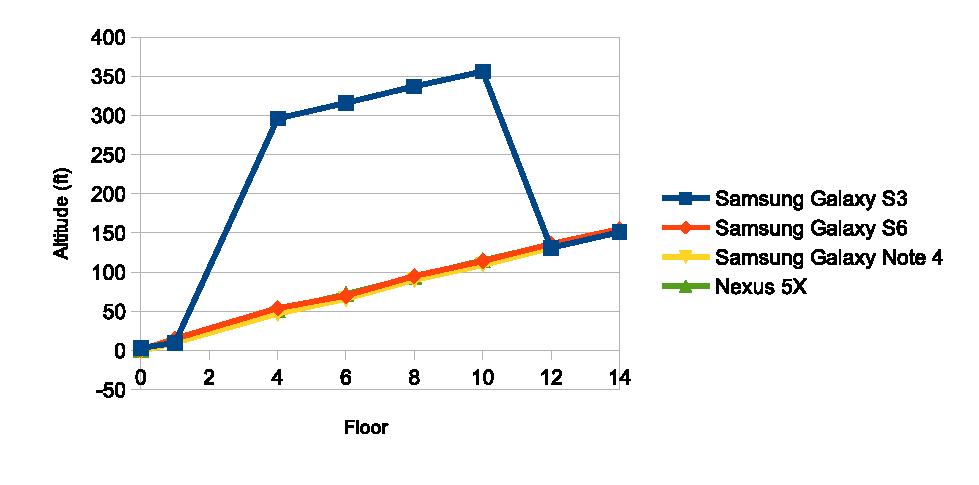
\includegraphics{alt-test-altitude}
    \caption{Altitude measurements from smartphones in Muirehead Tower}\label{fig:alt-test-altitude}
\end{figure*}

\begin{figure*}[h]
    \centering
    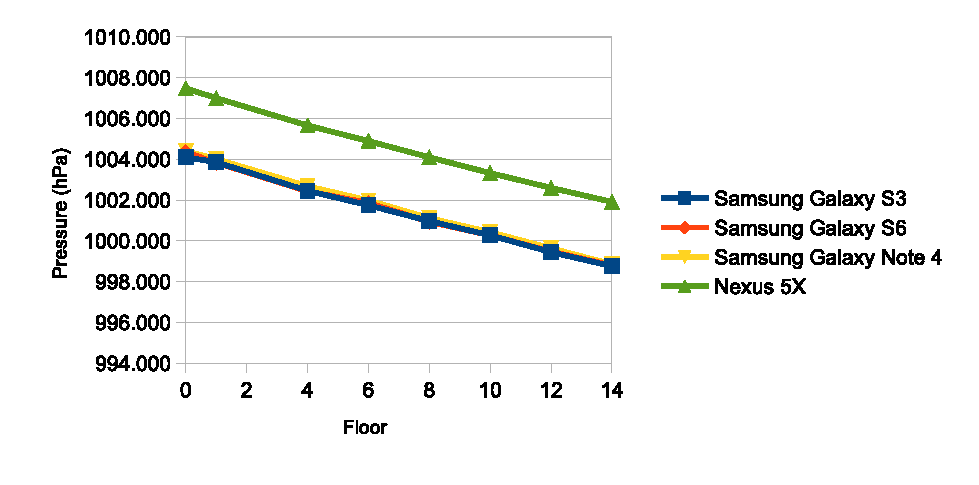
\includegraphics{alt-test-pressure}
    \caption{Air pressure measurements from smartphones in Muirhead Tower}\label{fig:alt-test-pressure}
\end{figure*}

Measurements for altitude were in feet since this is the most common unit used for skydiving in the UK and what the conventional altimeter was set to display. The skydiving altimeter that was used as a reference, unfortunately, could only be used on the top floor due to it resetting to zero if it does not detect altitude changes under a certain height. On the top floor of the building the skydiving altimeter that displays altitude in tens of feet showed a height of \SI{150}{\feet}, all smartphones showed similar readings between \SIlist{150; 160}{\feet}, as seen in Figure~\ref{fig:alt-test-altitude}.
Figure~\ref{fig:alt-test-pressure} shows that all phones follow the same rate of change in air pressure as the test moved down the floors of the building, however, the Nexus 5X appears to give higher pressure readings than the other phones. The higher pressure reading from the Nexus 5X could be due to a difference in the barometric sensor's calibration, it is likely that the Samsungs all use the same chip or similar and that the Nexus phone uses a chip from a different manufacturer.
There does seem to be some strange behaviour in the Galaxy S3's results, shown in Figure~\ref{fig:alt-test-altitude}. The altitude reading from the Galaxy S3 jumps from \SI{131}{\feet} to \SI{356}{\feet} between floors ten and eight (twelve and ten in the graph), which is not correct. Something must have changed in either the reference pressure or temperature to have caused this unexpected behaviour because when we look at results for the Galaxy S3 in Figure~\ref{fig:alt-test-pressure}, there are no strange jumps in the data. After testing again and not being able to reproduce the problem, it is entirely possible that this was due to a hard to activate bug in the test app. The test app was set up to track altitude data from GNSS as a source however many of the devices could not receive a satellite signal from within the building. The phones that could receive a GNSS signal verified previous research suggesting substantial inaccuracies in GNSS altitude data, often fluctuating by \SI{\pm10}{\feet}.

% Tested Wi-Fi Direct connection speed. Approx 4secs including time to click accept connection
Another test that has been conducted was to determine the typical time to establish a connection via Wi-Fi Direct. Three different phones were used to connect to each other across a room and timed until the word ``Connected'' showed on the screen. The time for a connection to be established across devices was approximately four seconds, including time to click ``Accept'' for the connection. Wi-Fi Direct connection times were tested to ensure that they are not too slow for the purposes we require.

% Discussion of justification for work
% Shows that smartphones may be appropriate for aiding skydivers
The altitude test has undoubtedly helped prove that today's smart devices are capable of measuring altitude to a useful degree of accuracy. Our findings were closely matched by a very similar test documented by \textcite{he_atmospheric_2012}. It is important to note that while the results are positive for demonstrating the appropriateness of using smart devices for altitude detection in some cases, this may not necessarily apply to the more extreme circumstances of skydiving.

% GNSS is inaccurate
That the GNSS data could not be used for a significant portion of the test, demonstrates why it would not be a suitable primary source for altitude data, smart devices would have to rely on having satellite signal which may not always be the case. On top of this, the altitude data provided by GNSS is inaccurate, we saw large, regular fluctuations in the altitude data produced.

% Discussion of experiments planned with justification
% Collection of data for testing
Other experiments are planned to verify certain aspects of the app. Sensor data will be collected from a few skydives that can be input into test harness programs to carry out these experiments and conduct A/B testing to find improvements without having to jump out of a plane every time.

% Test live landing pattern router
Firstly, once the live landing pattern feedback has been implemented, it must be tested. To test this, test data from previous skydives will be used and modified to see how the app performs with both expected user behaviour and unexpected user behaviour. The app should be able to direct the user to their landing area in all conditions where possible, and performance will be measured regarding how close to the centre of the landing area the user lands and how safe the instructions were.

% Test accuracy of barometers during freefall
Testing the accuracy of smart device barometers during freefall could prove to be very useful. The main features of the app concentrate on the user while under canopy, however, if barometer accuracy is good during freefall, the app could be extended to provide useful features for that part of a skydive too. We do have access to a skydiving altimeter that logs altitude for the whole period of a skydive. We will use this altimeter to compare data collected from a smart device that will also be set up to log altitude data, to establish how accurate it is during freefall. The closer the altitude data of the smart device is to the real skydiving altimeter, the better. Ideally, the difference between the smart device and the skydiving altimeter's altitudes will be less than \SI{10}{\metre}.

% Test range of Wi-Fi direct
It may be hard to test the range of Wi-Fi direct under canopy without putting people in danger, which is not something we are willing to do. Instead, the range can be tested in an open space such as a park by having two devices that start out of range of each other. The two devices should be moved towards each other until a connection is made between them. At the point of connection, the distance between the devices can be measured using GNSS coordinates to establish the range. The result may differ slightly from what may be achieved in the sky since for example clouds in the path between the devices could reduce the range of a connection.

% Data collection to investigate how much data we can track and effect on battery life
For optimisation purposes, experimentation could be done to find balances between logging and calculating all data and performing actions less frequently to improve battery life. By tracking battery levels and CPU usage, we can see how much stress we are putting the device under with different settings to be able to make conclusions on what needs to be changed to make the app more practical for users. The app would not be convenient for a user if it drained their battery during a skydive and so a balance must be found.

% Discussion of expected evaluation approach (final experiments)
The final evaluation of the app will measure success based on a few criteria; the first will be whether the app can successfully improve a skydiver's landing pattern and aid them in reviewing their jump. The second criteria are whether the app can carry out its functions without adding any risk to the skydiver. The final criteria for the performance of the app are that it should improve the safety of the skydiver. To evaluate the app based on these criteria, we will use the app during a skydive, following the landing pattern directions that the app gives. The app will be rated based on how close the skydiver is to their intended landing area and whether this would be an improvement when compared to a struggling student's landing. We will also test the landing pattern guidance tool programmatically, feeding it unexpected flight data to test for cases where an unsafe instruction may be given. To test that the app can increase skydiver safety, the app will be given to professionals that will fly their canopies close to each other to prompt a warning. This warning check will be done with an increased warning distance so that the canopies do not have to fly too close to test the feature. Alternatively, if no one can do the collision warning experiment in the sky, the same test can be done in an open area on the ground. Since we also want the app to be a useful tool for reviewing a jump, the app must also be able to log and playback location data and statistics from a jump to the user.

\section{Conclusion}\label{sec:conclusion} % Summarises research, discusses its significance

% The field
Little research has been conducted into the appropriateness of smart devices for safety-critical extreme sports such as skydiving. Research into smartphone barometers has been primarily for detecting static altitudes in a building and not for high-speed descents.

% Briefly restate project description
Instead of creating tools to teach skydivers only on the ground, we set out to create an aid for skydivers in the form of an Android app that can assist them during a skydive based on the current environment. The app will be able to help improve a skydiver's landing accuracy, provide useful information to learn from and communicate with other instances of the app to increase safety.

% Original motivation repeated

% State of the field in light of this paper reassessed
We hope that in light of this project, more people will consider the use of smart devices to assist in extreme altitude sports such as skydiving. An increase in the accessibility of advanced tools in sports where prices are high, and development is lagging is much needed to make use of our smart devices as they become more advanced and reliable.

\printbibliography{}
\end{document}
